% ===============================
% Biology of the house mice
% ===============================
\newpage
\section{Biology of the house mouse}
\label{sec:biolhousemice}

\subsection{Introduction}
\label{subsec:introduction}

House mice (\textit{Mus domesticus}) (see figure \ref{fig:housemice}) live under a multitude of different environmental conditions. The ecological success of house mice as a widely distributed species reflects the fact, that they are very flexible in terms of their social, territorial and reproductive behavior \citep{bronson:79, bronson:84, berry:81}. Under natural conditions house mice have a relatively low expectancy of life (100 to 150 days). During this short life span, female mice are avid to have as many offspring as possible. Living under optimal food conditions, a female mouse gives birth to a litter of 5-7 pups every four weeks \citep{berry:71, pelikan:81}. The juvenile mortality is estimated between 50\% and 85\% \citep{berry:71, berry:75, pennycuik:86}. Having heavier pups is an advantage, as they can be weaned faster, which positively influences future reproduction of the mother\citep{fuchs:82}. The litter size of a wild house mouse increases from the first to the second lactation and decreases after the fifth lactation \citep{pelikan:81, koenig:87b}. 

\begin{figure}[htbp]	
\centering	
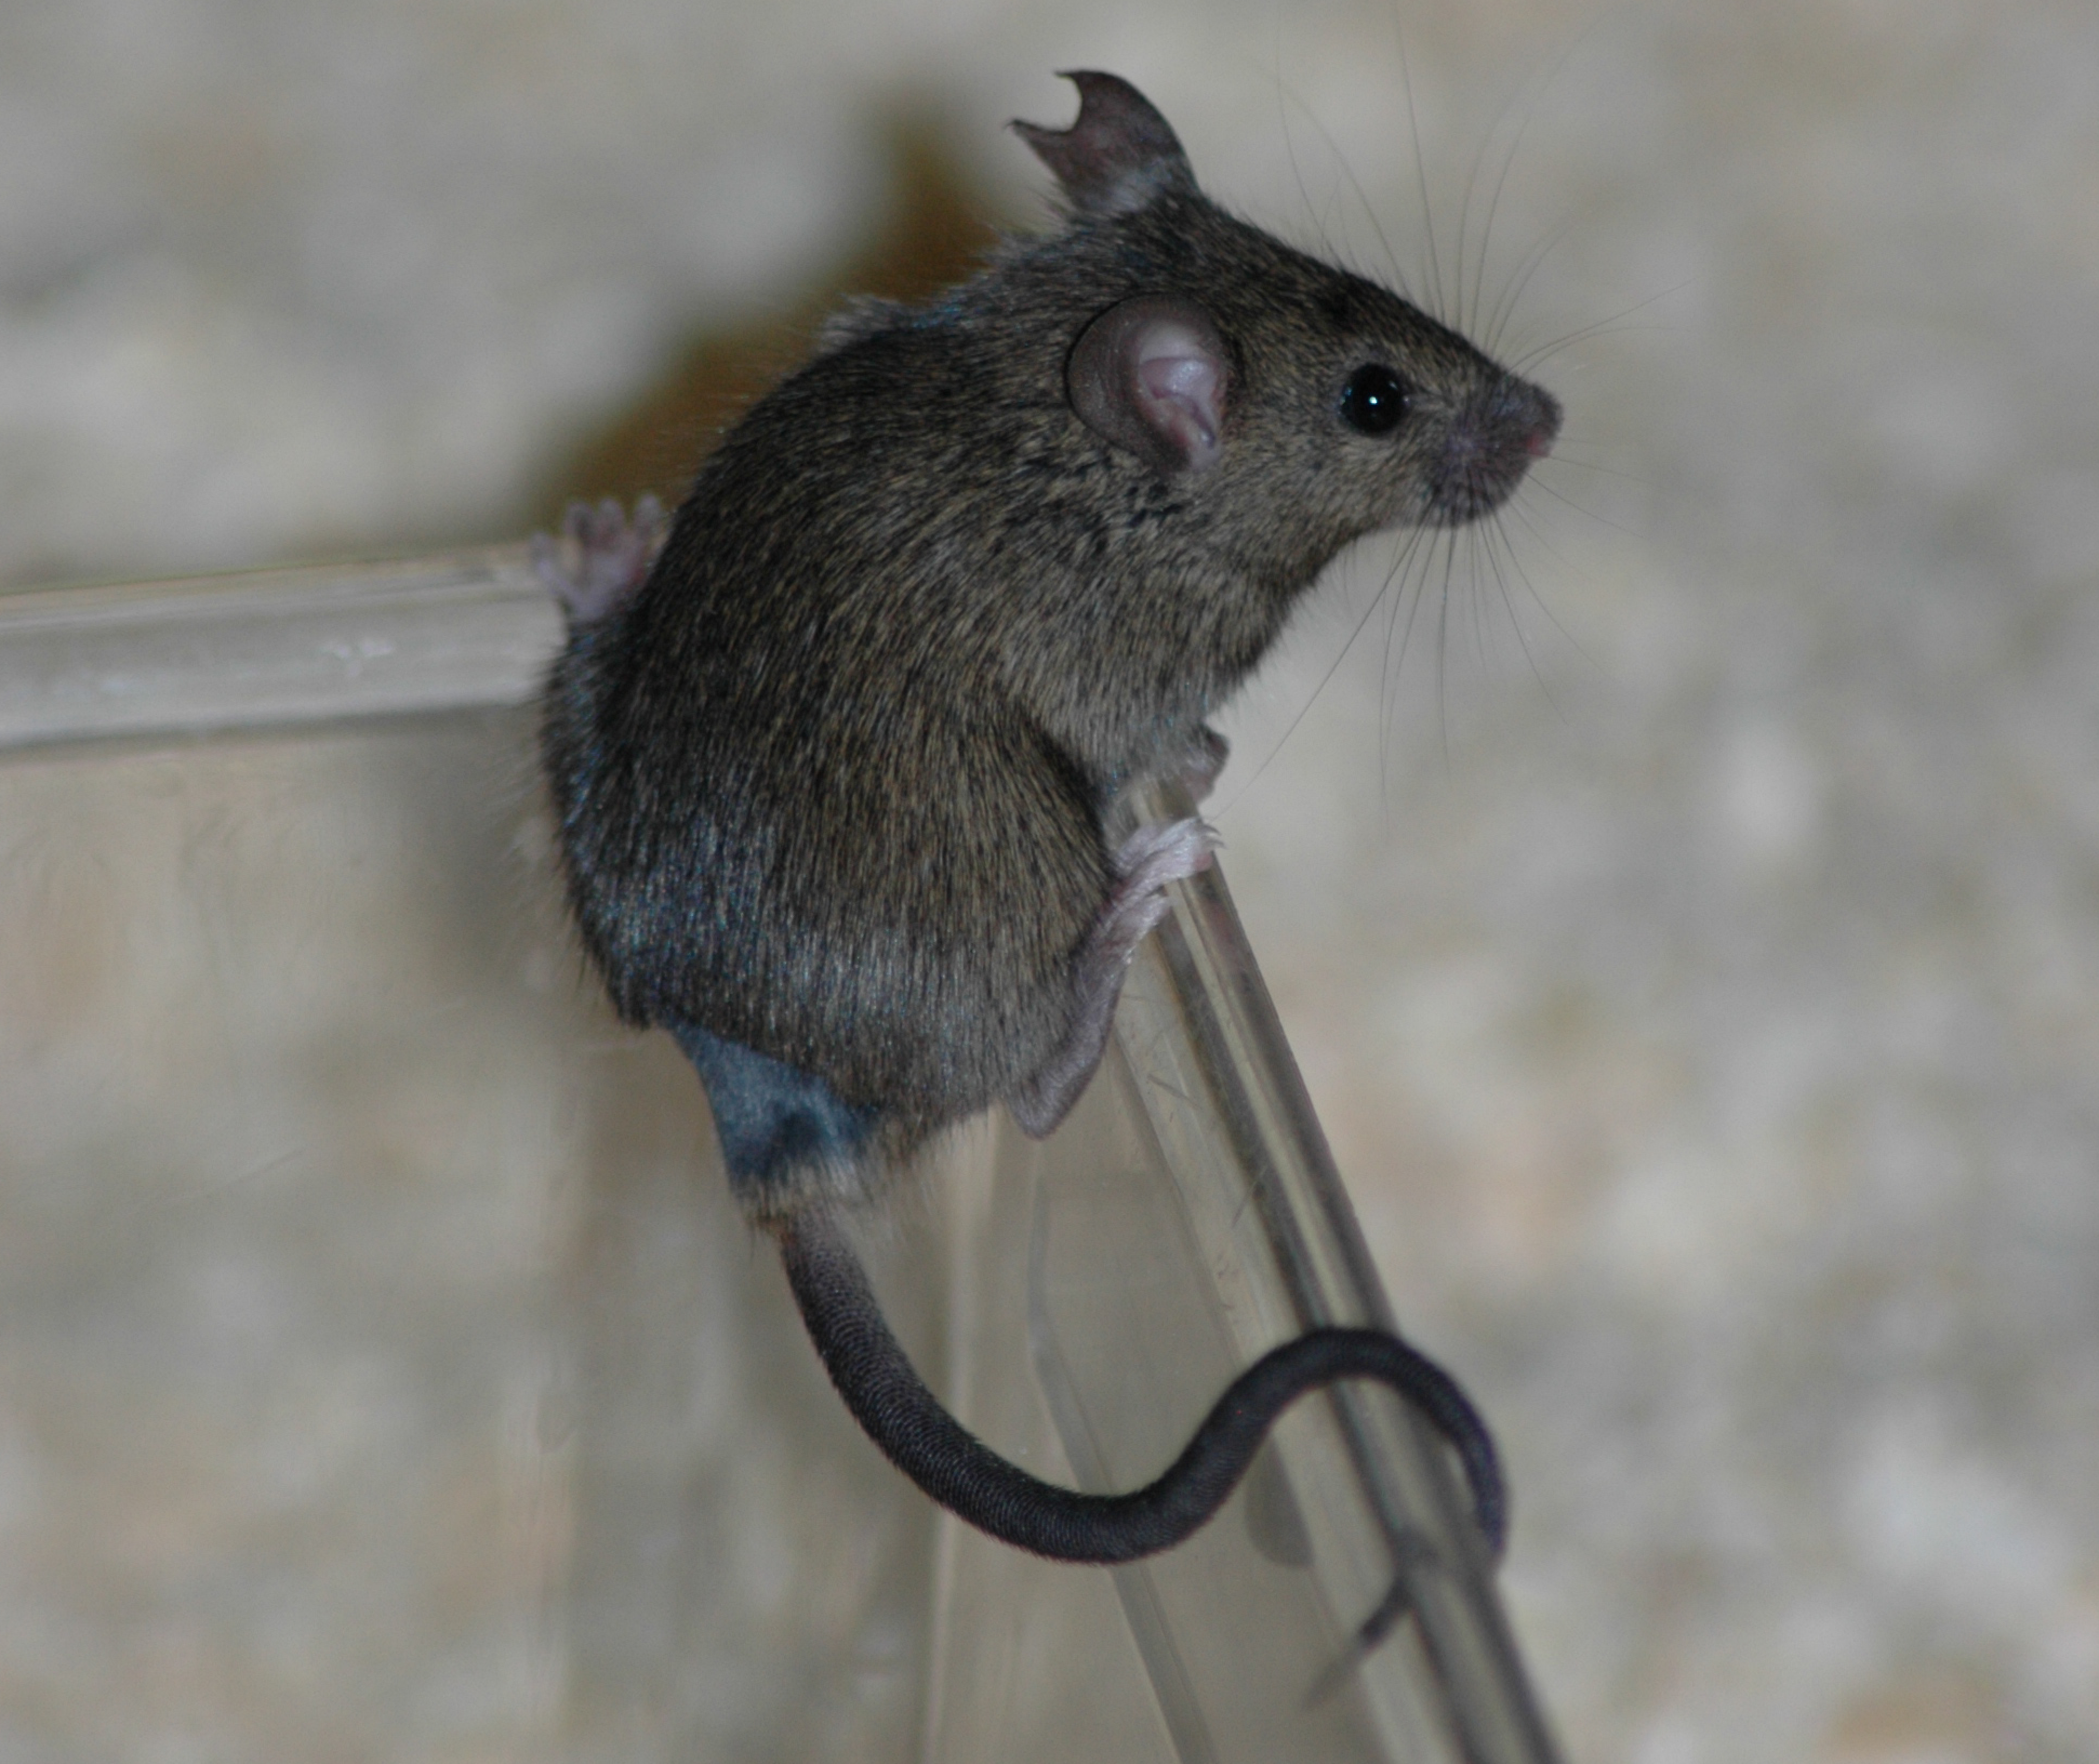
\includegraphics[width=0.5\textwidth]{assets/pdf/mus_domesticus.pdf}	
\caption[House mouse]{House mouse \textit{(Mus domesticus)}}
\label{fig:housemice}
\end{figure}

\subsection{General social behavior}
\label{subsec:socialbehaviour}
House mice typically live in a social collective which forms a reproduction group. These groups usually include a dominant male, one or several females with their litters and possibly some subordinate males \citep{crowcroft:63, reimer:67, selander:70, mackintosh:81}.

The mating habit is typically polygynandric (both males and females have several mating partners), but monogamic living pairs have also been reported \citep{lidicker:76}. Juvenile females may stay in the territory of their parents to raise their own offspring \citep{petras:67}. There is evidence of stranger females immigrating into social groups as well \citep{anderson:65, reimer:67, selander:70, bronson:79, baker:81}.     

\subsection{Research topics}
\label{subsec:researchtopics}

The research group in animal behavior around Prof. K\"onig at the University of Z\"urich is generally interested in the complex social behavior of the house mice. Mainly the influence of the social partner choice, other then mating, onto the fitness of the female mice, is in the focus of the studies. Such social selection occurs, if social interactions result in favorable fitness consequences. Therefore, reproductive cooperation such as joint nesting, for example, should manifest in an increased number of offspring \citep{weidt:07}. Cooperative interactions can extend to sharing of broad-rearing duties like nursing.

\subsubsection{Communal nursing}
\label{subsubsec:comnurs}

Over forty years ago, first observations of wild female house mice, belonging to the same reproduction group, which raise their pups in communal nests have been reported \citep{southwick:55}. Ever since, this behavior has been noticed for house mice living under all kind of environmental conditions.\citep{crowcroft:63, sayler:69, gandelman:70, werboff:70, baker:81}.

This behavior is astonishing, as the energetic costs of lactation are very high, hence influence the females' future reproduction success. To wean a litter of about seven to eight pups, the mother has to produce 100 grams of milk within 22 days, which is equivalent to 1100 \acf{KJ} \citep{koenig:88}. Depending on the size of the litter and the duration of the lactation phase, the length of the interbirth intervals change \citep{fuchs:81, fuchs:82, koenig:87a, koenig:87b}.

Several experiments have been carried out with wild house mice living under laboratory conditions. Manipulating group size and the composition of the group in terms of relatedness of the individuals revealed that non-offspring nursing is an integral part of the reproductive behavior of female house mice in egalitarian groups. However, the probability for such mutualistic cooperation was highest when a female shared a nest with a familiar sister to form a low-skew society \citep{koenig:06}.

According to K\"onig \citep{koenig:06}, the direct benefits of allomaternal care for the pups could be diverse. As there are, improved survival, improved future reproduction, improved growth or immunological benefits.

There are physiological benefits for the mother as well, which lead to an increase of their reproductive output. Of notable interest is the hypothesis named \textit{Metabolic peak load reduction}. Explained in short, a solitary nursing female tends to have a peak of energy consumption during the nursing phase of her litter. Nevertheless, female house mice are limited in their maximal sustainable metabolism \citep{hammond:92}. This limit depends on the age and physique of the individual and is called \textit{metabolic ceiling}. Partial synchronization in reproduction within the females of a group, combined with the communal nursing, can balance the energy demand for the individual, as the burden of nursing the litter is divided. Hence, the energy demand for each female stays always on a medium level\citep{koenig:06}. This can result in an increased lifetime reproduction success.

However, due to the artificial setup of the experiments, no conclusion about the communal nursing under natural conditions could be made.
